\section{Detalizuotas vertės grandinės modelis} \label{section:dvcm}

\BPMN modelyje galima pastebėti įmonės valdymo veiklų supratimo neapibrėžtumus \cite{bpmnPorterModel}. Taip yra todėl, kad išorinio modeliavimo metodai neparodo informacijos arba resursų transformavimo priežasčių. Tačiau įmonę galima analizuoti ir transakcinių darbų sekų modelio (\ref{img:pdca} pav) požiūriu.  
\begin{figure}[H]
	\centering
	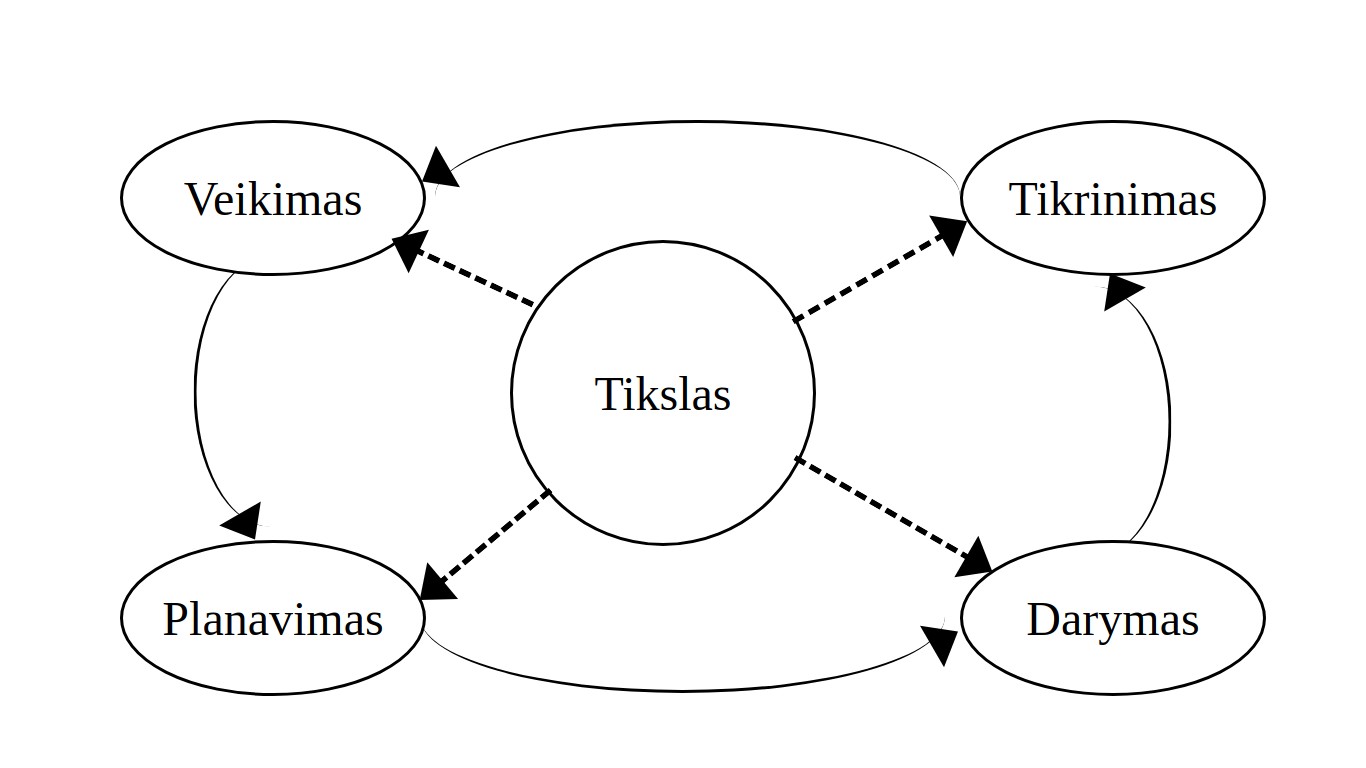
\includegraphics[width=10cm]{img/pdca}
	\caption{Transakcinių darbų sekų modelio pavyzdys}
	\label{img:pdca}
\end{figure} 

Darbe įmonės procesas bus nagrinėjamas kaip transakcijų visuma. Materialios veiklos atskiriamos nuo valdymo veiklų. $P_i$ žymi veiklos procesą, kuris transformuoja žaliavas, medžiagas, energiją ir formuoja materialią išeigą. $F_j$ yra veiklos valdymo funkcija, informacijos (duomenų, žinių) transformavimo veikla, būtina valdant procesą $P_i$. Modelis yra suskirstytas į valdymo transakcijas $ MT_{ij} = F_j \times P_i$. Tokiu būdu pateikiama daugiau informacijos apie įmonę. Diagrama bus vaizduojama kaip detalizuotas M. Porterio vertės grandinės modelis (\ref{img:detalized_porter_vcm} pav).

%TODO: show goles in diagram
\begin{figure}[H]
	\centering
	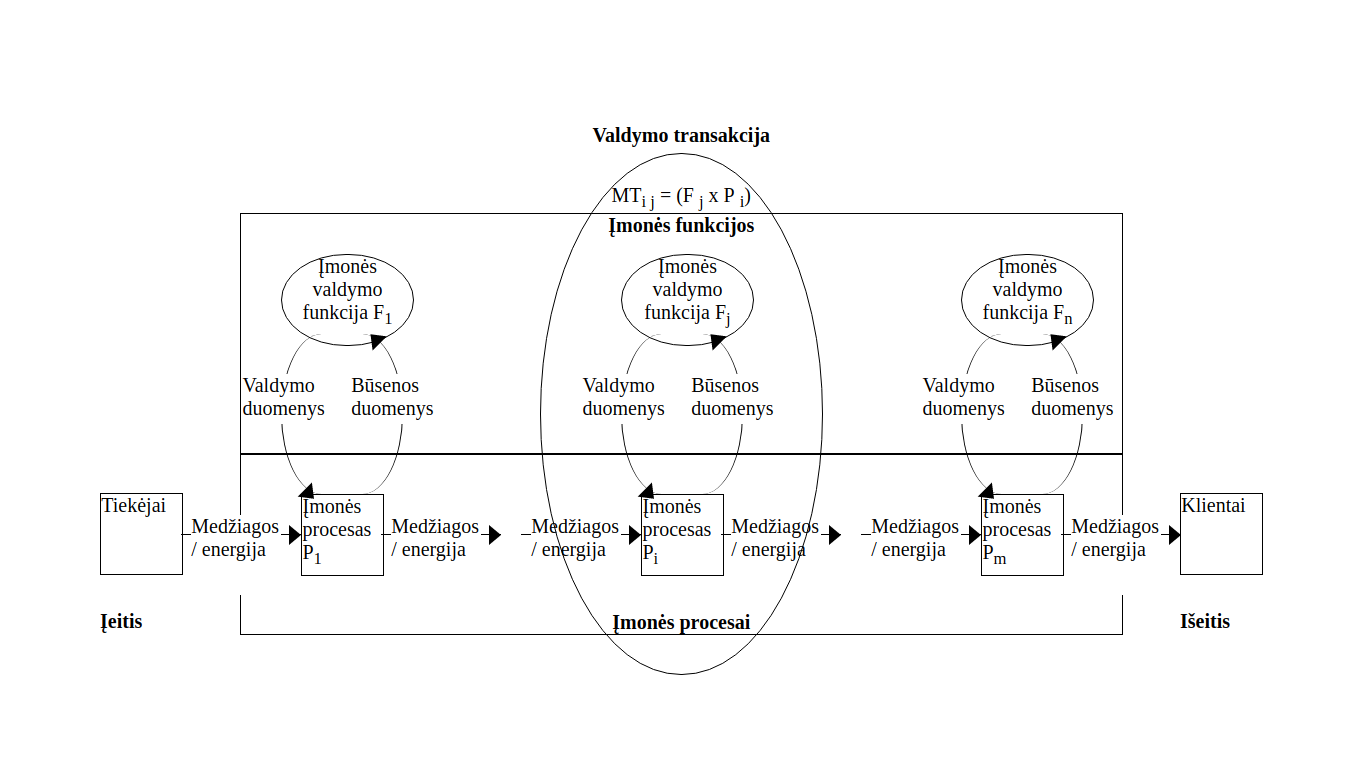
\includegraphics[height=8cm]{img/detalized_porter_vcm}
	\caption{Detalizuotas M. Porterio vertės grandinės modelis}
	\label{img:detalized_porter_vcm}
\end{figure} 

Valdymo funkcija $F_j$ gali būti suskaidyta smulkiau. (\ref{img:splitted_management_function} pav) parodytas pavyzdys kai $F_j$ susideda iš smulkesnių dalių $F_{j1}$, $F_{j2}$ ir $F_{j3}$. Kartu visa tai suteikia veiklos procesui $P_i$ valdymo duomenis kuriuos jis panaudoja vykdymui. Vėliau grąžinami būsenos duomenys, jie panaudojami valdymo funkcijoje ir ciklas kartojasi.

\begin{figure}[H]
	\centering
	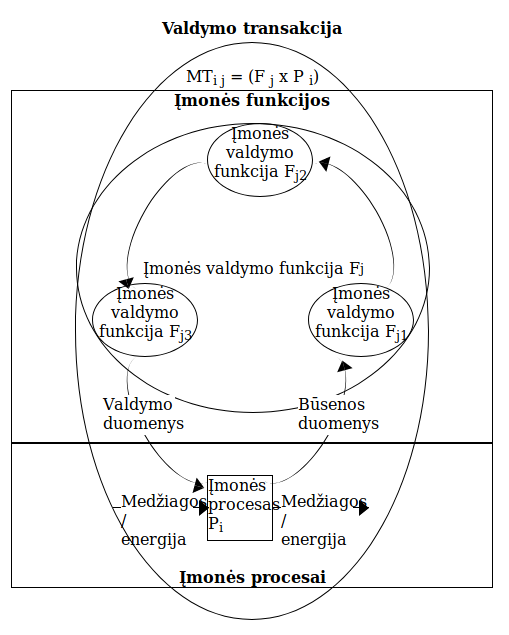
\includegraphics[width=7cm]{img/splitted_management_function}
	\caption{Valdymo funkcijos $F_j$ išskaidymo pavyzdys}
	\label{img:splitted_management_function}
\end{figure} 


\subsection{Detalizuoto vertės grandinės modelio apimtis}

Detalizuotas vertės grandinės modelis leidžia modeliuoti įmonės veikimą kaip transakcijų visumą. Jis atskiria vadybos veiklas nuo produkcijos veiklų. Parodomi valdymo informacijos ciklai, kurie kontroliuoja produkcijos veiklą ir padeda siekti įmonės užsibrėžtų tikslų. Taip pat parodomi informacijos srautų tipai, produkcijos veiklų įeigos ir išeigos tipai. Visa tai leidžia suprasti kodėl įmonėje egzistuoja viena ar kita valdymo transakcija ir kaip jos įtakoja įmonės tikslų pasiekimą.

\subsection{Detalizuoto vertės grandinės modelio komponentai}

\DVCM yra \BPMN modelio praplėtimas, suskirstantis įmonės veiklą į valdymo transakcijas ir atskiriantis valdymo funkcijas nuo įmonės procesų. Šiame modelyje galima naudoti komponentus iš \BPMN, taip pat pridedama keletas naujų. Iš pat pradžių yra dvi juostos: valdymo funkcijų vykdytojai ir įmonės procesų vykdytojai, kurie gali būti skaidomi smulkiau naudojant linijas.

\begin{figure}[H]
	\centering
	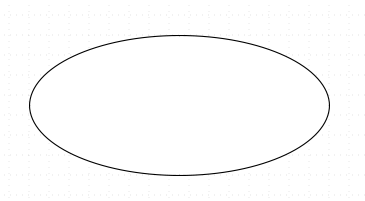
\includegraphics[height=2cm]{img/dvcm_components/management_function}
	\caption{Valdymo funkcijos pavyzdys}
	\label{img:dvcm_components_management_function}
\end{figure} 

Valdymo funkcija (management function) darbas atliekamas organizacijoje, kuris prisideda į valdymo duomenų generavimą. Šio darbo įeiga paprastai savyje turi jo valdomo įmonės proceso proceso būseną. Tai yra \BPMN veiklos komponento praplėtimas. Žymimas ovalu viduje paliekant vietos pavadinimui (\ref{img:dvcm_components_management_function} pav.).

\begin{figure}[H]
	\centering
	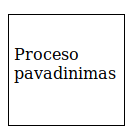
\includegraphics[height=2cm]{img/dvcm_components/process}
	\caption{Įmonės proceso pavyzdys}
	\label{img:dvcm_components_process}
\end{figure}

Įmonės procesas arba tiesiog procesas (process) yra darbas atliekamas organizacijoje, kuris tiesiogiai prisideda prie organizacijos gaminamos išeigos sukūrimo. Šis komponentas valdomas valdymo funkcijų per valdymo transakcijose keliaujančius duomenis. Joms jis pateikia savo būsenos duomenis ir gauna valdymo duomenis. Tai yra \BPMN veiklos komponento praplėtimas. Žymimas stačiakampiu viduje paliekant vietos pavadinimui (\ref{img:dvcm_components_process} pav.).

\begin{figure}[H]
	\centering
	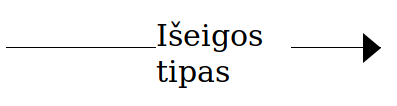
\includegraphics[height=1cm]{img/dvcm_components/sequence_flow}
	\caption{Interakcijų sekos srauto pavyzdys}
	\label{img:dvcm_components_sequence_flow}
\end{figure}

Interakcijų sekos srautas (interactions sequence flow) yra sekos srauto išplėtimas nurodant kas perduodama iš vienos veiklos į kitą. Kadangi įmonės veikla vaizduojama ciklais veiklos išeiga tampa kitos veiklos įeiga. Šis komponentas vaizduojamas solidžia linija su užpildyto trikampio formos rodykle gale ir išeigos (kuri tampa įeiga) tipo vardu prie pavaizduotos linijos (\ref{img:dvcm_components_sequence_flow} pav.). 

\begin{figure}[H]
	\centering
	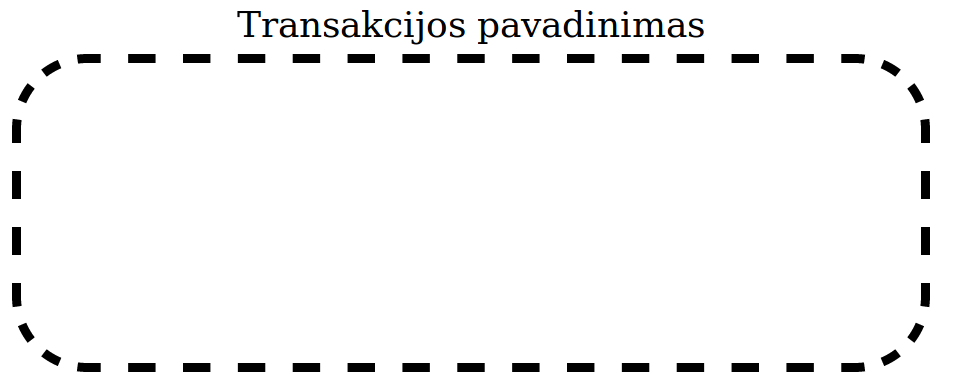
\includegraphics[height=2cm]{img/dvcm_components/management_transaction}
	\caption{Valdymo transakcijos pavyzdys}
	\label{img:dvcm_components_management_transaction}
\end{figure}

Valdymo transakcija (management transaction) yra grupė, kuri parodo, kaip valdymo funkcijos kontroliuoja įmonės procesą. Šis komponentas žymi valdymo duomenų transformacijų ciklą. Jis vaizduojamas punktyrine linija apibraukiant veiklas priklausančias transakcijai ir parašant transakcijos pavadinimą (\ref{img:dvcm_components_management_transaction} pav.). 

\subsection{Detalizuoto vertės grandinės modelio komponentų tarpusavio ryšiai}

\DVCM komponentų tarpusavio ryšiai pavaizduoti metamodeliu (\ref{img:dvcm_metamodel} pav.). Jis sudarytas panaudojant komponentus iš prieš tai sudaryto \BPMN metamodelio (\ref{img:bpmn_metamodel} pav.), jie pažymėti priešdėliu „BPMN::”.

\begin{figure}[H]
	\centering
	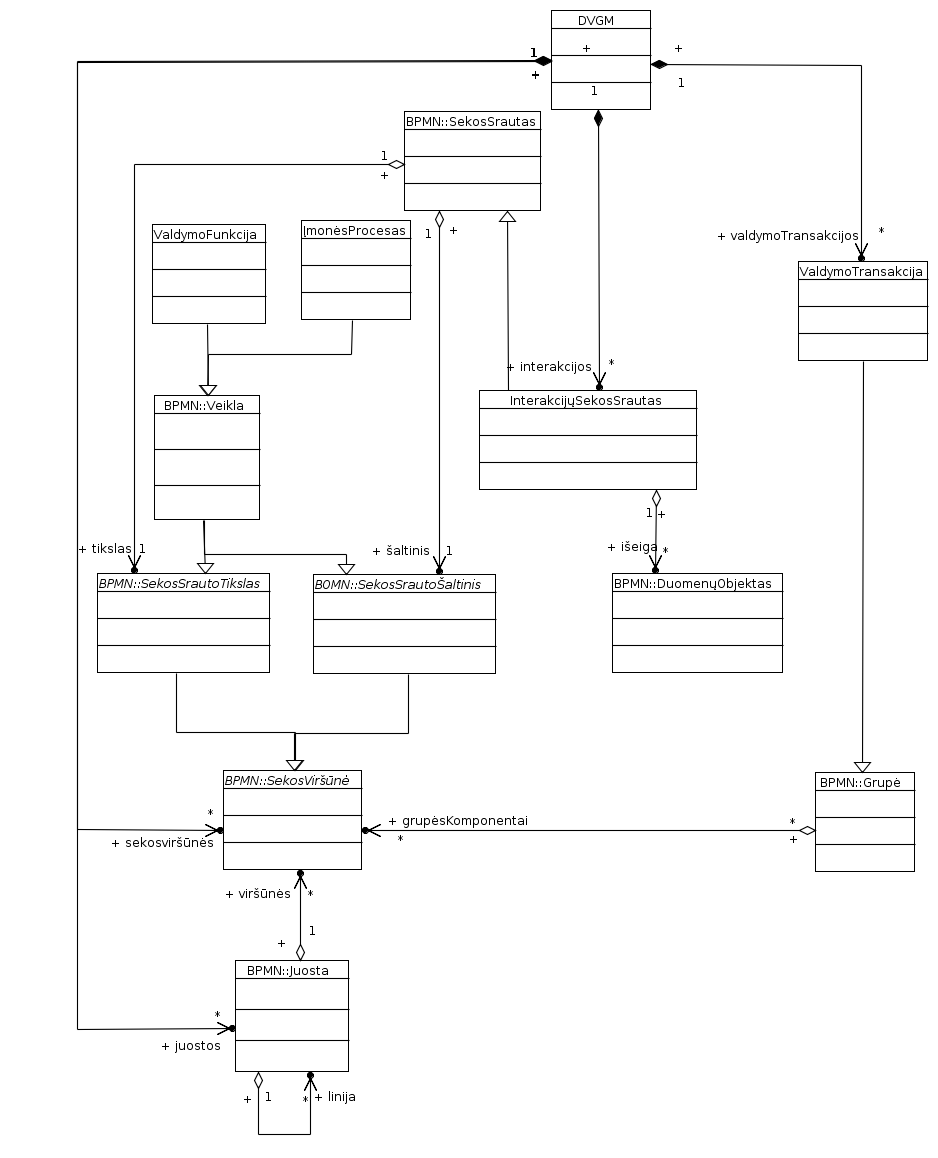
\includegraphics[width=12cm]{img/dvcm_metamodel}
	\caption{\DVCM metamodelis}
	\label{img:dvcm_metamodel}
\end{figure}

Šakninis komponentas \DVCM savyje laiko valdymo transakcijas, interakcijų sekos srautus, juostas ir sekos viršūnes. Valdymo funkcijos ir įmonės procesai yra sekos viršūnės. Jos gali būti interakcijų sekos srautų tiek šaltiniu tiek tikslu. Interakcijų sekos srautas savyje taip pat laiko duomenų objektą, kuris nurodo išeigos tipą. Valdymo transakcija yra grupė kuriai priklauso valdymo funkcijos ir įmonės procesai. Juostos gali būti skaidomos į linijas, jos savyje turi valdymo transakcijas ir įmonės procesus.
